%! ~~~ Packages Setup ~~~ 
\documentclass[]{article}
\usepackage{lipsum}
\usepackage{rotating}


% Math packages
\usepackage[usenames]{color}
\usepackage{forest}
\usepackage{ifxetex,ifluatex,amssymb,amsmath,mathrsfs,amsthm,witharrows,mathtools,mathdots}
\usepackage{amsmath}
\WithArrowsOptions{displaystyle}
\renewcommand{\qedsymbol}{$\blacksquare$} % end proofs with \blacksquare. Overwrites the defualts. 
\usepackage{cancel,bm}
\usepackage[thinc]{esdiff}


% tikz
\usepackage{tikz}
\usetikzlibrary{graphs}
\newcommand\sqw{1}
\newcommand\squ[4][1]{\fill[#4] (#2*\sqw,#3*\sqw) rectangle +(#1*\sqw,#1*\sqw);}

\usepackage[colorlinks]{hyperref}

% code 
\usepackage{listings}
\usepackage{xcolor}

\definecolor{codegreen}{rgb}{0,0.35,0}
\definecolor{codegray}{rgb}{0.5,0.5,0.5}
\definecolor{codenumber}{rgb}{0.1,0.3,0.5}
\definecolor{codeblue}{rgb}{0,0,0.5}
\definecolor{codered}{rgb}{0.5,0.03,0.02}
\definecolor{codegray}{rgb}{0.96,0.96,0.96}

\lstdefinestyle{pythonstylesheet}{
	language=Java,
	emphstyle=\color{deepred},
	backgroundcolor=\color{codegray},
	keywordstyle=\color{deepblue}\bfseries\itshape,
	numberstyle=\scriptsize\color{codenumber},
	basicstyle=\ttfamily\footnotesize,
	commentstyle=\color{codegreen}\itshape,
	breakatwhitespace=false, 
	breaklines=true, 
	captionpos=b, 
	keepspaces=true, 
	numbers=left, 
	numbersep=5pt, 
	showspaces=false,                
	showstringspaces=false,
	showtabs=false, 
	tabsize=4, 
	morekeywords={as,assert,nonlocal,with,yield,self,True,False,None,AssertionError,ValueError,in,else},              % Add keywords here
	keywordstyle=\color{codeblue},
	emph={var, List, Iterable, Iterator},          % Custom highlighting
	emphstyle=\color{codered},
	stringstyle=\color{codegreen},
	showstringspaces=false,
	abovecaptionskip=0pt,belowcaptionskip =0pt,
	framextopmargin=-\topsep, 
}
\newcommand\pythonstyle{\lstset{pythonstylesheet}}
\newcommand\pyl[1]     {{\lstinline!#1!}}
\lstset{style=pythonstylesheet}

\usepackage[style=1,skipbelow=\topskip,skipabove=\topskip,framemethod=TikZ]{mdframed}
\definecolor{bggray}{rgb}{0.85, 0.85, 0.85}
\mdfsetup{leftmargin=0pt,rightmargin=0pt,innerleftmargin=15pt,backgroundcolor=codegray,middlelinewidth=0.5pt,skipabove=5pt,skipbelow=0pt,middlelinecolor=black,roundcorner=5}
\BeforeBeginEnvironment{lstlisting}{\begin{mdframed}\vspace{-0.4em}}
	\AfterEndEnvironment{lstlisting}{\vspace{-0.8em}\end{mdframed}}


% Deisgn
\usepackage{nonfloat}
\usepackage[margin=0.6in]{geometry}
\usepackage{multicol}
\usepackage[skip=4pt, indent=0pt]{parskip}
\usepackage[normalem]{ulem}
\forestset{default}
\renewcommand\labelitemi{$\bullet$}
\usepackage{titlesec}
\titleformat{\section}[block]
{\fontsize{20}{40}}
{\large\dotfill \huge(\thesection)\large \dotfill}
{0em}
{\vspace{2pt} \newline \hfil \Large \filleft \filright \MakeUppercase}
\usepackage{graphicx}
\graphicspath{ {./} }
\definecolor{mgreen}{RGB}{25, 160, 50}
\definecolor{mblue}{RGB}{30, 60, 200}
\usepackage{hyperref}
\hypersetup{
	colorlinks=true,
	citecolor=mgreen,
	linkcolor=black,
	urlcolor=mblue,
	pdftitle={AI Something},
	pdfpagemode=FullScreen,
}


% Hebrew initialzing
\usepackage[bidi=basic]{babel}
\PassOptionsToPackage{no-math}{fontspec}
\babelprovide[main, import, Alph=letters]{hebrew}
\babelprovide[import]{english}
\babelfont[hebrew]{rm}{David CLM}
\babelfont[hebrew]{sf}{David CLM}
\babelfont[english]{tt}{Monaspace Xenon}
\usepackage[shortlabels]{enumitem}
\newlist{hebenum}{enumerate}{1}

% Language Shortcuts
\newcommand\en[1] {\begin{otherlanguage}{english}#1\end{otherlanguage}}
\newcommand\sen   {\begin{otherlanguage}{english}}
	\newcommand\she   {\end{otherlanguage}}
\newcommand\del   {$ \!\! $}

\newcommand\npage {\vfil {\hfil \textbf{\textit{המשך בעמוד הבא}}} \hfil \vfil \pagebreak}
\newcommand\ndoc  {\dotfill \\ \vfil {\begin{center}
			{\textbf{\textit{שחר פרץ, 2025}} \\
				\scriptsize \textit{קומפל ב־}\en{\LaTeX}\, $\sim$ \textit{ נוצר (בעיקר) באמצעות תוכנה חופשית }}
	\end{center}} \vfil	}

\newcommand{\rn}[1]{
	\textup{\uppercase\expandafter{\romannumeral#1}}
}

\makeatletter
\newcommand{\skipitems}[1]{
	\addtocounter{\@enumctr}{#1}
}
\makeatother

\newtheorem{Theorem}{משפט}
\theoremstyle{definition}
\newtheorem{definition}{הגדרה}
\newtheorem{Lemma}{למה}
\newtheorem{Remark}{הערה}
\newtheorem{Notion}{סימון}

\newcommand\theo  [1] {\begin{Theorem}#1\end{Theorem}}
\newcommand\defi  [1] {\begin{definition}#1\end{definition}}
\newcommand\rmark [1] {\begin{Remark}#1\end{Remark}}
\newcommand\lem   [1] {\begin{Lemma}#1\end{Lemma}}
\newcommand\noti  [1] {\begin{Notion}#1\end{Notion}}

\newcommand\s{$\sim$\ }

%! ~~~ Document ~~~

\author{שחר פרץ}
\title{\textit{הערכה חילופית בלשון $\sim$ על החשיבות והיכולות של Generative AI $\sim$ מאמר}}
\begin{document}
	\maketitle
	\tableofcontents
	
	\npage
	\section{מבוא}
	\begin{multicols}{2}
		\subsection{הגדרת הנושא והטיעון}
		בטיעון זה ארצה להדגים מדוע יש יותר מדי "הייפ" והתלהבות מיותרת ולא פורפורציונלית סביב נושא הבינה המלאכותית (AI). לשם כך, אתעסק עם השאלות הבאות: 
		\begin{itemize}
			\item מה בינה מלאכותית מסוגלת לעשות היום, ומה תהיה מסוגלת לעשות בעתיד? 
			\item כיצד נעריך "הייפ" והתלהבות, בצורה מדידה שתאפשר לנו להראות שאכן מדיתה אינה פורפורציונית למציאות? 
			\item מה כן ההשפעות של בינה מלאכותית, בהשוואה לאירועי עבר? 
		\end{itemize}
		הטיעון יבנה בצורה הבאה: 
		\begin{itemize}
			\item סיפוק רקע נרחב שיאפשר לנו להבין את הנושא לעומק. נגדיר "רקע" כנושא שלא מתעסק ישירות באחד או יותר מהנושאים לעיל. פרקים 1-4. 
			\item קישור הרקע לנושא, והסקת מסקנות – פרקים 5-6. 
			\item סיכום והוכחת הטענה – פרק 7. 
			\item ביבליוגרפיה – פרק 8. 
		\end{itemize}
		
		\subsection{מטרה}
		מטרת הטיעון הזה היא להוכיח באופן בלתי ניתן לערעור את הטענה. לכן, לא אפעל באופן רטורי בשביל רטוריקה, כי אין זה עוזר למטרה זו. זאת בניגוד למצגת שאציג בכיתה, שמטרתהּ לשכנע בדבר הנכונות. המצגת תהיה משכנעת ומתומצתת, בניגוד למאמר הזה המהווה להיות מסמך טכני, מפורט ופורמלי. 
		
		\subsection{רקע לוגי ותיאור המתודות להוכחת טענות}
		לפנות כל, ארצה להציג רעיונות תיאורטיים גרידא. הם חיוניים על מנת להגדיר (ואף באופן מקוצר) את כללי ההסק שישמשו כחוקיים. 
		
		ב־28 במרץ 2024, הורשע סם בנקמן־פריד (מעתה ואילך יקרא "SBF") בהונאות משקיעים בעולם הקריפטו בסכומים של מיליארדי דולרים, ונאסר ל־25 שנה \cite{SBF}. לאורך המשפט, SBF טען שהשתמש בכוחו כדי להפוך את העולם למקום יותר טוב. מראיונות קודמים, הובן כי SBF תמך בגישות תועלתניות מסויימות שגרמו לו לחשוב כי הבעיה המרכזית של האנושות היא המקום בכדו"א והסיכון שהאנושות תשמיד אותו, וכי הוא מכיר בבעיה ועל כן מוסרי עליו לפעול בדרכים לא חוקיות, ששוללות את הזכות של אנשים לבחירה חופשית על כיצד ישתמשו בממונם, כדי להשקיע בפתרון הבעיה \cite{SBFU}.
		
		אחת מן הנקודות הרבות שנראות לוגיות־לכאורה במחשבה זו, אך למעשה מתבססות על כללים שבורים, היא ההנחה כי נוכל לבצע (באמצעות כלים סבירים חישובית) היסק באמצעות כלים דטרמינסטיים על \href{https://he.wikipedia.org/wiki/%D7%AA%D7%95%D7%A8%D7%AA_%D7%94%D7%9B%D7%90%D7%95%D7%A1}{מערכת כיאוטית} כדוגמת האנושות והיקום כולו – הלוא דברים "פשוטים" כמזג האוויר, או שלוש מטוטלת, מתנהג באופן לא ליניארי וכאוטי. כמעט ולפי הגדרה, ניאלץ להיעזר בקירובים למערכת האמיתית (שמטבעם יהיו לא מדוייקים), או, במקרה העדיף – לחזות את התקדמות המערכת באופן \href{https://he.wikipedia.org/wiki/%D7%94%D7%99%D7%95%D7%A8%D7%99%D7%A1%D7%98%D7%99%D7%A7%D7%94}{היורסטי} (נסיוני) על בסיס התנהגותה בעבר. 
		
		על כן, בטיעון זה, רעיונות תיאורטיים־גרידא יחשבו כחסרי משמעות, אלא והינם מתארים מערכת מתמטית סופית דטרמיניסטית (כדוגמת מחשבים). נקראם \textbf{טיעונים מסוג ראשון}. על פניהם, נעדיף מחקרים המראים נתונים סטטיסטיים, או התבוננות באירועי עבר מוכרים היסטורית. נקראם \textbf{טיעונים מסוג שני}. מהסיבות שראינו בפרק זה – טיעונים מסוג ראשון תמיד יוכלו להיות מופרכים ע"י טיעונים מסוג שני. נפריד טיעונים מסוג שני לשני סוגי טיעונים – כאלו המתבססים על מחקרים על טווח זמן קצר (בהתחשב באופי הנושא שעלה רק בשנים האחרונות – כל טיעון מחקרי שיובא כאן) וכאלו המתבססים על היסטוריה ארוכת טווח. מנימוקים דומים טיעוים היסטורים יחשבו כחזקים מטיעונים מחקריים. 
		
		\subsection{טרמינולוגיה}
		במהלך העבודה אשתמש במספר מושגים שלא מן העברית – ולכן, שום שזו עבודה בעברית, בעבור אלו שאשתמש בהם הרבה, אגדיר מקבילה עברית (והאמת, אולי גם קצת כדי לצחוק על האקדמיה ללשון העברית, שכן באמת ובתמים קשה לקרוא את המשפט 'מש"ג מורכב מקשבים וקר"שים'). באופן דומה אגדיר תעתיק של שמות:
	\end{multicols}
	
	\begin{center}
		\begin{tabular}{|c|c|c|c|}
			\hline אנגלית & קיצור אנגלי & עברית & קיצור עברי \\
			\hline Artificial Intelligence & AI & בינה מלאכותית & ב"מ \\
			\hline Generative AI & GenAI & ב"מ מחולל & במ"מ \\
			\hline Nvidia & - & אנבידיה & - \\
			\hline Large Language Model & LLM & מודל שפה גדול & מש"ג \\
			\hline Overvalueation & - & הערכת יתר & - \\
			\hline Multilayer Perceptron & MLP & קולטן רב־שכבתי & קר"ש \\
			\hline Attention & - & קשב & - \\
			\hline Interpolation & - & ביון & - \\
			\hline Bias & - & נטאי & - \\ 
			\hline Intellectual Property & IP & קניין רוחני & ק"ר \\
			\hline Optimization & - & כילול & - \\
			\hline Integration & - & מיטוב & - \\
			\hline
		\end{tabular}
	\end{center}
	
	
	\npage
	
	\section{רקע היסטורי}
	\subsection{בועת הדוט־קום}
	\begin{multicols}{2}
		בשנים 1995 ל־2001 התפתחה בועה כלכלית שנקראה בועת־קום. משמעותה של בועה כלכלית היא שאנשים קונים קניין בערך יותר גבוהה מהערך האמיתי שלו, במחשבה שערכו גבוהה יותר \cite{bubble}. לדוגמה, אם תצפה שחברה תשלש את הכנסותיה בשנתיים הקרובות, תקנה את מנייתה ע"פ ההנחה הזו במחיר משולש ממה שהיה ללולא קצב גידול הכנסותיה היה נותר אותו הדבר. 
		
		בועת הדוט־קום התאפיינה בהערכת יתר של חברות העוסקות באינטרנט, שהיה חדש בתקופה. נפריד בין שני סוגים של חברות: 
		\begin{itemize}
			\item חברות "מסוג 1" שמרוויחות כסף ממשי מהתקיימות הבועה, לדוגמה, באמצעות מכירת שירותים במחירים גבוהים לחברות ואנשים פרטיים אחרים;
			\item חברות "מסוג 2", שלא עם הכנסות נמוכות, ועדכן נקבע ע"פ הצפי שיגדילו הכנסות בקרוב. 
		\end{itemize}
		דוגמה לחברה מסוג 2 יכולה להיות וואטסאפ (טרם נקנתה) – מטא ציפתה שתוכל להפוך את מיליארדי משתמשיה לרווחיים (שכן באותה התקופה לא היה מודל כלכלי) ועל כן קנתה אותה ב־22 מיליארד דולר, בציפייה שתוכל לנצל את בסיס משתמשים זה. דוגמה לחברה מסוג 1 היא סיסקו, בזמן בועת הדוט־קום – היא סיפקה את תשתיות האינטרנט לכל העולם, עם מונופול חסר עוררין באותה התקופה. נתבונן בגרף הבא ביחס לסיסקו באותה התקופה:
		
		
		\begin{minipage}{\linewidth} 
			\centering
			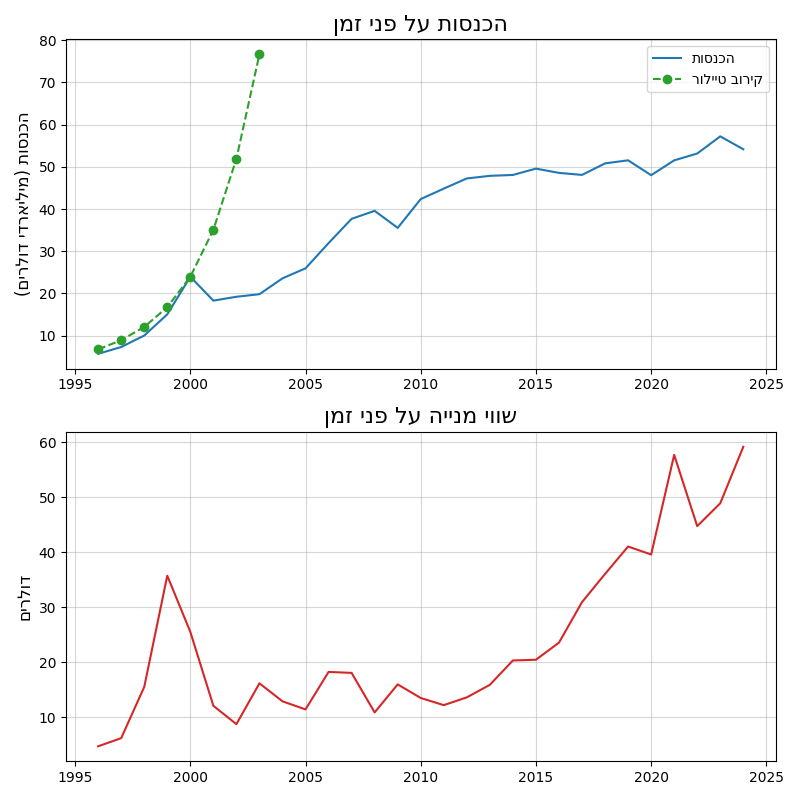
\includegraphics[width=\linewidth]{../cisco_revenue/revenue+taylorapprox}
			\figcaption{מניית ורווחי סיסקו בשנים 1996-2024 \cite{CSCOstock}\cite{CSCOrevenue}}
			\label{fig:input.eps}
		\end{minipage} 
		
		נבחין שעד שנת 2000 (ליתר דיוק, אמצע 2001) רווחי סיסקו גדלו בקצב מעריכי. השתמשתי באלגוריתם שכתבתי (ליתר דיוק, טור טיילור דיסקרטי מסדר 5) בשביל לחזות את הכנסות סיסקו במידה והיו ממשיכים בקצב בו המשיכו עד שנת 2000.
		
		התפוצצות הבועה, והקריסה הכלכלית של החברות מהסוג הראשון (שכן הן לא ייצרו כסף והסתמכו על כסף ממשקיעים בשביל להישאר באוויר) שהיו לקוחותיהם העיקריים שלהם, הובילו לירידה חדה במכירות. 
		
		
		מספר החברות מהסוג השני לרוב מועט, כי בעולם הטכנולוגיה, לרוב למספר קטן של חברות יש מונופול על סיפוק תשתית לחברות אחרות (נאמר, בתחום המעבדים הגרפים – אנבידיה בלבד. בתחום בענן – גוגל, אמזון ומיקרוסופט בלבד. בתחום ה־virtualization – בעיקר VMWare, וכו'). לכן, נוכל לנצל את ההסתכלות על מחיר המנייה והרווח של חברה מסדר שני בזמן בועה כלכלית בשביל להסיק מה השוק צופה בעבור העתיד בתחום (פונ' של מחיר המניה) ומה גודל השוק עכשיו (פונ' של ההכנסות). תחת ההנחה שכל חברה מסוג 1 תצטרך תשתיות מחברה מסוג 2 ביחס ישר להשקעתה בתחום, אותה הפונ' תהיה ליניארית. 
		
		נותר לנו דבר אחד שחסר להשלמת הפאזל – ההבנה אם אותן חברות מסוג 1 באמת יצליחו לייצר הכנסות בעתיד, או שרק יתפסו נתח שוק. נדבר על כך בהרחבה בהמשך. 
		
		יש לציין, שבמקרים מסויימים נוכל למצוא חברות הן מסדר 1 והן מסדר 2, מה שיקשה על בידוד משתנים. נתעסק גם עם בעיה זו בהמשך. 
		
		לסיכום, כדי לקבוע אם אנו מצויים בבועה כלכלית, נתייחס לנקודות הבאות: 
		\begin{itemize}
			\item מה גודל השוק (מה גודל הבועה) – באמצעות המתודות לעיל. לא דרוש להוכחת קיום, אלא רק להבנת גודל הבעיה. 
			\item מה הצפי לגדילת השוק – באמצעות המתודות לעיל. 
			\item כמה השוק באמת שווה, וכמה כסף יוכל להכניס – נתעסק בבעיה זו בהמשך. 
		\end{itemize}
	\end{multicols}
	
	\npage
	
	\section{רקע טכנולוגי}
	
	\subsection{על המושגים}
	נסביר בקצרה את המושגים שהובאו בפרק 1.4. ניעזר במילון אוקספורד \cite{OxfordDict}. 
	\begin{itemize}
		\item בינה מלאכותית – מחקר ופיתוח מערכות מחשב שמדמות התנהגות אנוש. 
		\item בינה מלאכותית מחוללת – בינה מלאותית שמחקה התנהגות אנושית, ויוצרת חומרים חדשים. 
	\end{itemize}
	להגדרה הרחבה יותר של בינה מלאכותית, נופלים אלגוריתמים פרימיטייבים יחסית רבים. בפרט, כל סוג של אינטרפולציה (ביון) או אפילו טור טיילור (כמו זה שכתבתי והשתמשתי בו בפרק 2.1). להגדרה הצרה יותר של במ"מ נכנסים מודלים כמו \en{GPT, Dall$\cdot$E, Claude}\,  וכו'. 
	
	כבר כאן נבחין בבעיה – איזה תוכן נחשב "חדש"? נתעסק בה רבות בפרק זה, כדי להבין לעומק את הבעיה במ"מים. 
	
	\subsection{מבוא קצר לפעילות מש"ג}
	יש לציין שטכנולוגיה הבמ"מים השונות עבודות באופן טיפה אחר. כדוגמה, נתבונן במש"ג – מודל במ"ח שמטרתו לחזות טקסט. 
	(מבוסס על סרטונים של 3Blue1Brown). 
	
	[מעובד קונספטואלית באופן שקול, כדי לא להכנס למימושים של דברים באלגברה ליניארית. וגם כי זה חרא קורס]
	
	במש"ג מילים מיוצגות באמצעות סדרה סופית של מספרים כלשהם, נקראם "וקטורים". נוכל להפריד את פעולת מש"ג לשני שלבים עיקריים: 
	\subsubsection{קשב}
	
	 הראשון, קשב. בהקשר הזה, תפקידה לקשר בין חלקים שונים במשפט. נרצה להשוות כל וקטור $v_i$ במשפט לוקטור $v_j$ אחר, בעבור איזשהו פרמטר $Q$ (לצורך הדוגמה, כמה "אדומות" שתי מילים או כמה "יפות" הן, $Q$ ינסה לקדד). נעביר את $v_i$ ו־$v_j$ דרך טרנספורמציות של $Q$, ונשווה את שני הוקטורים החדשים שקיבלנו מהטרנספומציה. ככל שהשינוי יותר קטן, ו־$v_i$ יותר דומה ל־$v_j$, נחבר ל־$v_i$ יותר מה"ערך" של $Q$. סה"כ קיבלנו $v_i'$ כלשהו, שהוא למעשה $v_i$ בתוספת השינוי של $Q$ ביחס לוקטור $v_j$. 
		
		נחזור על התהליך בעבור מספר רב של ערכי $Q$ (כמו להשוות את $v_i$ ל־$v_j$ במספר פרמטרים שונים), ועבור $v_i$ נשווה אותו לכל וקטור $\forall 1 \le j \le i \colon v_j$ (כלומר, לכל המילים הקודמות). 
		
		בכך המש"ג יוכל להבין מילים עם קונטסט – כלומר, כל מילה תהפוך לאחר שלבי ה־קשב למילה חדשה, עם קונטסט ביחס למילים קודמות. 
		
		כל טרנספורמציה וערך בתוך המודל לא ידועיים, עד שמתחילים לאמן את המודל – שם כל ערך $Q$ (על הטקנספורמציות והערכים שלו) מתכייל להיות משהו שנושא משמעות. 
		
		משום שמודלים כמו LLaMA 3.1 יכולים לדרוש כיול של חצי טריליון מספרים (פרמטרים) שונים, תהליך האימון ארוך, ודורש כוח מחשוב רב. המספרים האלו כוללים את הפרמטרים של שלב נוסף במש"ג – הקר"ש. 
	\subsubsection{קר"ש}
	השלב הזה נמצא בין כל "בלוק" של קשבים. בעבור כל וקטור שקיבלנו, נעביר גם אותו דרך טרנספורמציה (שכמו בשלב הקשב, יש לכייל אותה בזמן אימון המודל) שלאחריו תזרוק את כל הערכים מתחת לערך מסוים (יש לכייל גם אותו) הנקרא נטאי, 
	
	
	
	\subsection{יכולות מודלי במ"מ}
	
	בהתחשב בנאמר לעיל, במ"מ הוא "תיקון אוטומטי על סטרואידים" \cite{AutoCorrect} (ציטוט של לינוס טורבאלדס, המתחזק הראשי של לינוקס, מערכת ההפעלה הפופולארית בעולם) – יש לבמ"מ את היכולת "להבין" קונטקסט (קשב) ולהשוואות אותו לדברים שראה בעבר (קר"ש). אפשר להתסכל עליו באל ביון רב־ממדי ענקי, שמכיל בתוכו חלק ניכר מהידע האנושי. אך, אין לו כל יכולת לייצר באמת משהו חדש לחלוטין – שכן הוא לא כולל בפנים שום מנגנון שמנסה לדמות הסקה, פיתוח, או השתנות. במ"מים, במצבם הנוכחי, בהתאם לאלגוריתמים הנוכחיים שלהם, תמיד יוכלו להסתמך אך ורק ע"י המידע הקיים. 
	
	הגדלת במ"מ, בהקשר של הגדלת מש"ג, משמעותה אחד משניים: 
	\begin{itemize}
		\item הגדלת הקשבים – כך הב"מ תוכל לקשר בין כל מילה למספר רק יותר של מילים (וקטורים) שהופיעו לפניה. 
		\item הגדלת הוקטורים עצמם שמייצגים את המילים, מה שמאפשר לאצור בכל מילה יותר מידע. 
	\end{itemize}
	
	הגדלה של הוקטורים פי קבוע $c$ תגרור תוספת של $\Omega(c^{2.4})$ למספר הפרמטרים הכולל במודל (מהבינום של ניוטון וסיבוכיות כפל מטריצות), כלומר לכל הפחות גידול מערכי בעבור כל $c$ ערכים שמוסיפים. הגדלת בלוק קשב, יקרה אף יותר (למעשה ב־$\Omega(c^{4.8})$ לפחות). 
	
	[אלו חסמים תחתונים בלבד שחשבתי בעצמי – החסמים האמיתיים כנראה גבוהים יותר]
	
	\npage
	\section{רקע כלכלי}
	
	\subsection{השקעות תשתיתיות}
	הדבר האקראי שאבא נתן לי...
	
	\subsection{השקעה בחברות}
	
	\subsubsection{השקעות בחברות מסוג 1}
	אנבידיה...
	
	\subsubsection{השקעות בחברות מסוג 2}
	סטראטאפים, מיקרוסופט וכאלו. 
	
	\subsection{על הרווחים היום}
	לקשר למחקרים שמראים או לא מראים שיפור בפרודוקטיביות וכו'. 
	
	\npage
	\section{קישור הרקע לטענה המרכזית}
	\subsection{מסקנות ממצב הכלכלה}
	בהתחשב בכמות הכסף שנכנסת בשביל תשתיות, סטארטאפים וצבירת ק"ר, אפשר לקבוע שאנשים מתרגשים ביחס למה שב"מ תוכל לעשות בעתיד, בטוחים בהצלחתה, ומוכנים להשקיע בכך כסף. למעשה, הצלחנו למדוד "הייפ". 
	
	עם זאת, ראינו מצב איזומורפי ששקול לבועת הדוט־קום: חברות שמתעסקות בנושא, מקבלות כולן את כספן (וגם עם בעקיפין, כמו במקרה של חברות מסוג 2) מכספי משקיעים. זהו טיעון מסוג 2 – ראינו אירועי עבר דומים, ועתה אפשר לקבוע שהמצב איזומורפי, ועל כן התוצאה תהיה זהה. גם במקרה הזה, משקיעים רבים תולים תקוות בכך שחברות אלו יהפכו לרווחיות בעתיד, כלומר, המודלים שלהן ישתפרו מספיק כדי להפוך להיות יותר מועילים ולייצר הכנסות, שלאחר מכן יהפכו לרווחים. אך זהו אינו המצב;
	
	\subsection{מסקנות על יכולות עתידיות}
	נוכל למצוא שני דרכים לשפר את המודלים: 
	
	\subsubsection{שיפורים אלגוריתמיים}
	ההנחה שאלגוריתמי בינה מלאכותית ישתפרו לאורך השנים, היא הנחה שאי אפשר להסתמך עליה. באותה המידע שלא היה ניתן לחזות את מתי יתפתחו המודלים של הבמ"מים המותוארים בפרק 3.1, לא ניתן לחזות מתי יתפתחו מודלים חדשים לחלוטין שלא יוגבלו למגבלות המותארות בסעיף 3.3. וב"מ לא תוכל למצוא אלגוריתמים חדשים לבמ"מים מרוכבים יותר, מתוקף אותן מגבלות. 
	\subsubsection{שיפורים תשתיתיים}
	כמו שראינו בפרק 3.3, ע"מ להשיג כל שיפור ליניארי בבמ"מ, יש צורך להשיג שיפור מערכי בתשתיות שמריצות ומאמנות אותו. 
	
	כמו שראינו בפרק 4, אחת מהמגבלות העיקריות לפיתוח בינה מלאכותית הוא קצב גידול החומרה: 
	\begin{itemize}
		\item \textbf{חומרה: }עלויות חומרה היו צפויות לרדת באופן מעריכי כל עוד חוק מור היה בתוקף. חוק מור לא בתוקף יותר מכורח העובדות בשנים האחרונות. 
		
		\item \textbf{כילול ומיטוב: }על כן, נוכל לשפר את החומרה אך ורק באמצעות שיפורי ארכיטרטורה (אופן עיצוב השבבים) ומיטובי חומרה ברמת ה־low level (כלומר, ברמת הקוד שרץ ישירות על החומרה). מנכ"ל אנבידיה, שנמצא בניגוד אינטרסים בנושא, טען שכילוול של תשתית, ומיטוב ארכיטקטורה ותוכנה יוכלו להביא אף להתקדמות יותר מהירה מבחוק מור (שעובד במקדם של $\sqrt2$ לשנה) \cite{HuangLaw}. 
		
		הבעיה בטענה זו, היא שזוהו טיעון מסדר 2, אך חסר ביסוס היסטורי. כלומר, הטיעון לכשעצמו חסר משמעות ולא ניתן להוכחה; אי אפשר לטעון לבצע מיטוב וכילול לאורך מספר רב של שנים, בעבור דוגמה של שנה אחת של פיתוח. ברמה הפרקטית, לרוב יש גבול לכמות המיטובים שאפשר לבצע. [דרוש מקור]. 
	\end{itemize}
	
	סך הכל, אין בסיס עובדתי לכך שנוכל לבצע שיפורים מערכיים במהירות החומרה, מה שמהווה תנאי הכרחי לשיפור מערכי בתשתית. כלומר, נוכל לצפות לשיפור בסדר גודל של $o(n)$ (יותר קטן ולא הדוק מליניארי) בהסתכלות על מספר רב של שנים קדימה. עלויות בניית תשתית ועלויות חשמל מעולם לא ירדו באופן מעריכי וכן כנראה לעולם לא ירדו (אם כי השני מביניהם יכול להפתר בהנחה שיבוצעו כילול ומיטוב בסדר גודל מעריכי). 
	
	\subsection{צפי}
	להערכתי, בהתחשב הנאמר לעיל, אנחנו נמצאים בבועה כלכלית. היא תתפוצץ באחד משלושה המקרים: 
	\begin{itemize}
		\item חברות מסוג 2 יכשלו בלהראות גידול מעריכי ביכולות התשתית, או באופן שקול, חברות מסוג 1 יכשלו בלהראות שיפור ליניארי במודלים שלהם;
		\item חברות מסוג 1 יכשלו בלייצר הכנסות לאורך זמן, משקיעים יבחינו בכך שאותן חברות חסרות ערך, וכספיהם יפסיקו לממן את הבועה. 
		\item כמו בבועת הדוט־קום, אירועים חיצוניים (העלת ריבית, מלחמות וכו') יגרמו למשקיעים לחשוב שוב על השקעותיהם, ולהמנע מהשקעות מסוכנות יותר בחברות הזנק או בהבטחות מסוכנות מחברות גדולות יותר. 
	\end{itemize}
	
	\npage
	
	\section{קישור הרקע להפרכת טענות נגד}
	\subsection{מי אתה להתווכח עם אנשים שחכמים ממך?}
	\subsection{"AI זה העתיד"}
	\subsection{אז אתה אומר שצריך להפסיק להשקיע ב־AI?}
	
	\section{סיכום הדברים}
	
	\npage
	\section{ביבליוגרפיה}
	\begin{multicols}{2}
	\renewcommand{\section}[2]{}
	\en{\begin{thebibliography}{}
			\bibitem{SBF}
			U.S. department of justice (2025) $\sim$ \emph{Samuel Bankman-Fried Sentenced to 25 Years for His Orchestration of Multiple Fraudulent Schemes.} $\sim$ \href{https://www.justice.gov/archives/opa/pr/samuel-bankman-fried-sentenced-25-years-his-orchestration-multiple-fraudulent-schemes}{Link}
			
			\bibitem{SBFU}
			CONTEMPORARY UTILITARIANS $\sim$ \emph{Sam Bankman-Fried} \s \href{https://www.utilitarianism.com/sam-bankman-fried.html}{Link}
			
			\bibitem{bubble}
			Nasdaq $\sim$ \emph{Economic bubble} $\sim$ \href{https://www.nasdaq.com/glossary/e/economic-bubble}{Link}
			
			\bibitem{CSCOstock}
			macrotrends.net $\sim$ \emph{Cisco - 35 Year Stock Price History} $\sim$ \href{https://www.macrotrends.net/stocks/charts/CSCO/cisco/stock-price-history}{Link}
			
			\bibitem{CSCOrevenue}
			companiesmarketcap.com \s \emph{Revenue for Cisco (CSCO)} \s \href{URLhttps://companiesmarketcap.com/cisco/revenue/}{Link}
			
			\bibitem{OxfordDict}
			Oxford English Dictionary \s \href{https://www.oxfordlearnersdictionaries.com/}{Link}
			
			\bibitem{AutoCorrect}
			linux.slashdot.org \s  \emph{Linus Torvalds on 'Hilarious' AI Hype} \s \href{https://linux.slashdot.org/story/24/04/19/1944235/linus-torvalds-on-hilarious-ai-hype}{Link}
			
			\bibitem{HuangLaw}
			Frobes \s \emph{Can Nvidia’s ‘Hyper Moore’s Law’ Spark An AI Revolution?} \s \href{www.cosmico.org/jensen-huang-predicts-millionfold-compute-in-10-years/}{Link}
		\end{thebibliography}
	}
	\end{multicols}
	
	\npage
	\section{דברים נוספים}
	\subsection{כלים עיקריים}
	\begin{multicols}{2}
		\begin{itemize}
			\item יצירת המסמך: \hfill \en{\LaTeX}
			\item עריכת המסמך: \hfill \en{\TeX Studio}
			\item יצירת גרפים: \hfill \en{MatPlotLib, Numpy, Python 3.13}
			\item עורך קוד: \hfill \en{PyCharm}
			\item חיפוש מאמרים: \hfill \en{Google Scholar}
			\item דפדפן: \hfill \en{FireFox, Zen}
			\item קרנל: \hfill \en{The Linux Kernel}
			\item הפצה: \hfill \en{Arch$^{\text{btw}}$ Linux}
			\item כלים אקראיים של גנו בשביל שסטלמן יהיה שמח: \hfill \en{CoreUtils} \\
			("אבל זה מקומפל ב־GCC!!")
			\item ניהול חלונות: \hfill \en{Hyprland}
			\item כלים גנריים לסביבת העבודה: \hfill \en{Kitty Console, Okular, \\ Dolphin, Wofi, NeoVim, GwenView \hfill}
			\item מלחינים שהחזיקו אותי בחיים במהלך הכתיבה של הדבר הזה: \hfill \en{Prokofiev, Mahler, Schönberg, Richard Strauss, Nielsen, Liszt \hfill}
		\end{itemize}
	\end{multicols}
	
	\hfil \textbf{תודה לקהילת הקוד הפתוח והחופשי שגרמה לשני שליש מהתוכנות למעלה להתקיים}
	
	\subsection{ניגוד עניינים}
	אין ניגוד עניינים כי אני ילד בן 15 בלי כסף אישי ובלי השקעות. אני אפילו לא עובד. 
	
	\subsection{אודותי}
	אני שחר פרץ, סטודנט למדעי־המחשב באוניברסיטת תל־אביב, חבר בקבוצת הרובוטיקה "GreenBlitz", ותלמיד בכפר הירוק. 
	
	
	
	\ndoc
\end{document}